\documentclass[12pt,a4paper]{article}

% 使用中文宏包
%\usepackage[UTF8]{ctex}
\usepackage{authblk}
\usepackage{graphicx} %插入图片的宏包
\usepackage{float} %设置图片浮动位置的宏包
\usepackage[strings]{underscore}
\usepackage{times}
\usepackage{epsfig}
\usepackage{amsmath}
\usepackage{amssymb}
\usepackage{overpic}
\usepackage{listings}
\usepackage{color}
\usepackage{enumitem}
\setenumerate[1]{itemsep=0pt,partopsep=0pt,parsep=\parskip,topsep=5pt}
\setitemize[1]{itemsep=0pt,partopsep=0pt,parsep=\parskip,topsep=5pt}
\setdescription{itemsep=0pt,partopsep=0pt,parsep=\parskip,topsep=5pt}

\definecolor{mygreen}{rgb}{0,0.6,0}
\definecolor{mygray}{rgb}{0.5,0.5,0.5}
\definecolor{mymauve}{rgb}{0.58,0,0.82}
\lstset{ %
  backgroundcolor=\color{white},   % choose the background color
  basicstyle=\footnotesize,        % size of fonts used for the code
  breaklines=true,                 % automatic line breaking only at whitespace
  captionpos=b,                    % sets the caption-position to bottom
  commentstyle=\color{mygreen},    % comment style
  escapeinside={\%*}{*)},          % if you want to add LaTeX within your code
  keywordstyle=\color{blue},       % keyword style
  stringstyle=\color{mymauve},     % string literal style
}

\usepackage[pagebackref=true,breaklinks=true,letterpaper=true,colorlinks,bookmarks=false]{hyperref}


\def\httilde{\mbox{\tt\raisebox{-.5ex}{\symbol{126}}}}


\graphicspath{{figures/}}

\setcounter{page}{1}

\begin{document}


%%%%%%%%% TITLE

\title{Expediting Training Process of Rice Grading Neural Netowks Using Singular Value Decomposition}
\author[*]{Na Wenqi(22018000164)}
\author[*]{Chang Chengxia(22018000163)}
\date{}
\affil[*]{School of Information Science \& Engineering, Yunnan University}

\maketitle

\begin{abstract}
The abstract goes here.
\end{abstract}

\section{Introduction}

\section{Related works}

\section{Methods}
\paragraph{} In this section we will introduce the method for accelerating training of deep networks via using SVD in order to reduce the number of parameters of networks. According Figure \ref{Fig.model}, we will argue our method in three steps as follows.
	\begin{figure}[H]
		\centering
		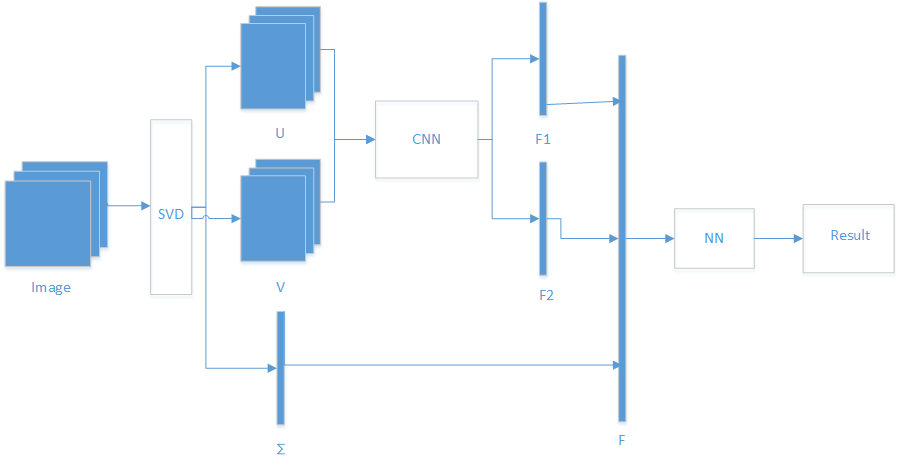
\includegraphics[width=0.7\textwidth]{../images/svd-cnn-arch.png}
		\caption{The neural network with SVD}
		\label{Fig.model}
	\end{figure}
	\subparagraph{} First of all, we assume that the size of the input images is $h\times w \times c$. Namely the image height is $h$, the width is $w$, and the count of channel is $c$. Before inputting the images into the neural network, we first perform singular value decomposition on the image. The Result of decomposition is three tensors: $U$, $V$, and $\Sigma$, and the dimensions of them are: $h\times r \times c$, $w \times r \times c$, $r\times 1 \times c$ respectively, where $r \ll h$ and $r \ll w$.
	\subparagraph{} We then stack the $U$ and $V$ before inputting them into our predefined convolutional neural network and obtain two vectors $F_1$ and $F_2$ through the convolutional layer and the flattened layer.
	\subparagraph{} Finally, overlaying $F_1$, $F_2$, and $\Sigma$ together to form a vector $F$, and then input $F$ into the final fully connected layer of the convolutional neural network to get the output.
\paragraph{} In this way, a large matrix input can be decomposed into two smaller matrices and a vector input. By adjusting the value of $r$, the number of parameters required by the neural networks can be controlled.

\section{Experiments}
\subsection{Dataset}
\paragraph{} We conduct our experiments using the FIST-Rice dataset. FIST-Rice is a multi-sensor based open rice grading dataset that includes approximately 30,000 samples taken from three angles by three high speed cameras, where samples are divided into two categories: sound kernels and unsound kernels.
\subsection{The Architecture}
\paragraph{} The introduction of SVD in the deep learning networks aims to reduce network parameters and shorten training time, thus improving training efficiency. How to design an effective deep learning network is not the main task of this paper. Therefore, in this paper, we implement the part of CNN and NN in the model based on VGG-16\cite{vgg}, and compare the plain VGG-16 network method and the VGG-16 method using SVD to illustrate the effect of the model.
\paragraph{} During the actual experiment process, one thing needs special attention. Since there are many convolutional layers in the VGG model, and the matrix dimensions obtained by SVD are relatively small, these matrix inputs into the CNN model will converge to the fully connected layer faster than the original image. Therefore, we need to adjust the size of the convolution kernels or reduce the number of convolutional layers to ensure that the algorithm performs correctly.
\paragraph{} The other issue that needs attention is that the singular value decomposition of the image consumes computational resources, which reduces computational efficiency and increases runtime. However, when we train a dataset, we usually perform dozens of epoches of training. At this time, if we cache the result of each image singular value decomposition, we do not need to perform singular value decomposition operation when repeating each epoch of calculation. Therefore, the operation time for singular value decomposition of an image can be regarded as a constant time, so that it is ignored when comparing computational efficiency.

\subsection{Results}
\paragraph{} By comparing the results of the experiments from the VGG model and the model proposed in this paper, we found that the nunber of the network parameters is about 8 million, when using the SVD model and letting $r=50$, which is less than the numbers of the parameters of the VGG-16 model(14 million) about 6 million. We can reduce by 57\% parameters from the VGG model. From the running time point of view, the VGG model runs for about 4300 seconds, and after using SVD, the proposed model runs for about 2800 seconds and the running time is reduced by about 35\%.

\section{Conclusion}
\paragraph{} Our work proposed a method to apply singular value decomposition to convolutional neural networks in order to reduce network parameters and accelerate the training process. This method can be applied to the training process of the FIST-Rice dataset, which can effectively improve the training efficiency. At the same time, this method can also be applied to other datasets or convolutional neural networks.

\paragraph{} There are currently two problems with this method. First of all, although this method can significantly reduce the network parameters and improve the efficiency from time to time, this method does not have any significant improvement on the classification accuracy of rice grading. In the case of improper training parameters, it will be counterproductive and the classification accuracy will be reduced. Another problem is that the convolutional neural networks are generally suitable for the case where the image height and width are approximated, and the two matrices $U$ and $V$ obtained by the singular value decomposition will have $r \ll h$ or $r \ll w$, so that $U$ and $V$ cannot be applied to deeper convolutional networks.
\paragraph{} The next step we will be doing is to find an approach not only to reduce network parameters but also to be proper to apply to convolutional networks, while at the same time not affecting the classification accuracy of the networks.





\bibliographystyle{ieeepes}
\bibliography{../Saliency}
\end{document}



























































